\documentclass[1p]{elsarticle_modified}
%\bibliographystyle{elsarticle-num}

%\usepackage[colorlinks]{hyperref}
%\usepackage{abbrmath_seonhwa} %\Abb, \Ascr, \Acal ,\Abf, \Afrak
\usepackage{amsfonts}
\usepackage{amssymb}
\usepackage{amsmath}
\usepackage{amsthm}
\usepackage{scalefnt}
\usepackage{amsbsy}
\usepackage{kotex}
\usepackage{caption}
\usepackage{subfig}
\usepackage{color}
\usepackage{graphicx}
\usepackage{xcolor} %% white, black, red, green, blue, cyan, magenta, yellow
\usepackage{float}
\usepackage{setspace}
\usepackage{hyperref}

\usepackage{tikz}
\usetikzlibrary{arrows}

\usepackage{multirow}
\usepackage{array} % fixed length table
\usepackage{hhline}

%%%%%%%%%%%%%%%%%%%%%
\makeatletter
\renewcommand*\env@matrix[1][\arraystretch]{%
	\edef\arraystretch{#1}%
	\hskip -\arraycolsep
	\let\@ifnextchar\new@ifnextchar
	\array{*\c@MaxMatrixCols c}}
\makeatother %https://tex.stackexchange.com/questions/14071/how-can-i-increase-the-line-spacing-in-a-matrix
%%%%%%%%%%%%%%%

\usepackage[normalem]{ulem}

\newcommand{\msout}[1]{\ifmmode\text{\sout{\ensuremath{#1}}}\else\sout{#1}\fi}
%SOURCE: \msout is \stkout macro in https://tex.stackexchange.com/questions/20609/strikeout-in-math-mode

\newcommand{\cancel}[1]{
	\ifmmode
	{\color{red}\msout{#1}}
	\else
	{\color{red}\sout{#1}}
	\fi
}

\newcommand{\add}[1]{
	{\color{blue}\uwave{#1}}
}

\newcommand{\replace}[2]{
	\ifmmode
	{\color{red}\msout{#1}}{\color{blue}\uwave{#2}}
	\else
	{\color{red}\sout{#1}}{\color{blue}\uwave{#2}}
	\fi
}

\newcommand{\Sol}{\mathcal{S}} %segment
\newcommand{\D}{D} %diagram
\newcommand{\A}{\mathcal{A}} %arc


%%%%%%%%%%%%%%%%%%%%%%%%%%%%%5 test

\def\sl{\operatorname{\textup{SL}}(2,\Cbb)}
\def\psl{\operatorname{\textup{PSL}}(2,\Cbb)}
\def\quan{\mkern 1mu \triangleright \mkern 1mu}

\theoremstyle{definition}
\newtheorem{thm}{Theorem}[section]
\newtheorem{prop}[thm]{Proposition}
\newtheorem{lem}[thm]{Lemma}
\newtheorem{ques}[thm]{Question}
\newtheorem{cor}[thm]{Corollary}
\newtheorem{defn}[thm]{Definition}
\newtheorem{exam}[thm]{Example}
\newtheorem{rmk}[thm]{Remark}
\newtheorem{alg}[thm]{Algorithm}

\newcommand{\I}{\sqrt{-1}}
\begin{document}

%\begin{frontmatter}
%
%\title{Boundary parabolic representations of knots up to 8 crossings}
%
%%% Group authors per affiliation:
%\author{Yunhi Cho} 
%\address{Department of Mathematics, University of Seoul, Seoul, Korea}
%\ead{yhcho@uos.ac.kr}
%
%
%\author{Seonhwa Kim} %\fnref{s_kim}}
%\address{Center for Geometry and Physics, Institute for Basic Science, Pohang, 37673, Korea}
%\ead{ryeona17@ibs.re.kr}
%
%\author{Hyuk Kim}
%\address{Department of Mathematical Sciences, Seoul National University, Seoul 08826, Korea}
%\ead{hyukkim@snu.ac.kr}
%
%\author{Seokbeom Yoon}
%\address{Department of Mathematical Sciences, Seoul National University, Seoul, 08826,  Korea}
%\ead{sbyoon15@snu.ac.kr}
%
%\begin{abstract}
%We find all boundary parabolic representation of knots up to 8 crossings.
%
%\end{abstract}
%\begin{keyword}
%    \MSC[2010] 57M25 
%\end{keyword}
%
%\end{frontmatter}

%\linenumbers
%\tableofcontents
%
\newcommand\colored[1]{\textcolor{white}{\rule[-0.35ex]{0.8em}{1.4ex}}\kern-0.8em\color{red} #1}%
%\newcommand\colored[1]{\textcolor{white}{ #1}\kern-2.17ex	\textcolor{white}{ #1}\kern-1.81ex	\textcolor{white}{ #1}\kern-2.15ex\color{red}#1	}

{\Large $\underline{12n_{0816}~(K12n_{0816})}$}

\setlength{\tabcolsep}{10pt}
\renewcommand{\arraystretch}{1.6}
\vspace{1cm}\begin{tabular}{m{100pt}>{\centering\arraybackslash}m{274pt}}
\multirow{5}{120pt}{
	\centering
	\includegraphics[width=112pt]{../../../GIT/diagram.site/Diagrams/png/2905_12n_0816.png}\\
\ \ \ A knot diagram\footnotemark}&
\allowdisplaybreaks
\textbf{Linearized knot diagam} \\
\cline{2-2}
 &
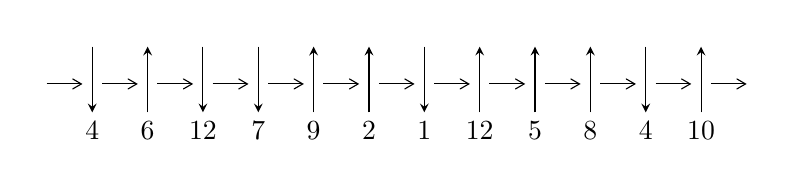
\begin{tikzpicture}[x=20pt, y=17pt]
	% nodes
	\node (C0) at (0, 0) {};
	\node (C1) at (1, 0) {};
	\node (C1U) at (1, +1) {};
	\node (C1D) at (1, -1) {4};

	\node (C2) at (2, 0) {};
	\node (C2U) at (2, +1) {};
	\node (C2D) at (2, -1) {6};

	\node (C3) at (3, 0) {};
	\node (C3U) at (3, +1) {};
	\node (C3D) at (3, -1) {12};

	\node (C4) at (4, 0) {};
	\node (C4U) at (4, +1) {};
	\node (C4D) at (4, -1) {7};

	\node (C5) at (5, 0) {};
	\node (C5U) at (5, +1) {};
	\node (C5D) at (5, -1) {9};

	\node (C6) at (6, 0) {};
	\node (C6U) at (6, +1) {};
	\node (C6D) at (6, -1) {2};

	\node (C7) at (7, 0) {};
	\node (C7U) at (7, +1) {};
	\node (C7D) at (7, -1) {1};

	\node (C8) at (8, 0) {};
	\node (C8U) at (8, +1) {};
	\node (C8D) at (8, -1) {12};

	\node (C9) at (9, 0) {};
	\node (C9U) at (9, +1) {};
	\node (C9D) at (9, -1) {5};

	\node (C10) at (10, 0) {};
	\node (C10U) at (10, +1) {};
	\node (C10D) at (10, -1) {8};

	\node (C11) at (11, 0) {};
	\node (C11U) at (11, +1) {};
	\node (C11D) at (11, -1) {4};

	\node (C12) at (12, 0) {};
	\node (C12U) at (12, +1) {};
	\node (C12D) at (12, -1) {10};
	\node (C13) at (13, 0) {};

	% arrows
	\draw[->,>={angle 60}]
	(C0) edge (C1) (C1) edge (C2) (C2) edge (C3) (C3) edge (C4) (C4) edge (C5) (C5) edge (C6) (C6) edge (C7) (C7) edge (C8) (C8) edge (C9) (C9) edge (C10) (C10) edge (C11) (C11) edge (C12) (C12) edge (C13) ;	\draw[->,>=stealth]
	(C1U) edge (C1D) (C2D) edge (C2U) (C3U) edge (C3D) (C4U) edge (C4D) (C5D) edge (C5U) (C6D) edge (C6U) (C7U) edge (C7D) (C8D) edge (C8U) (C9D) edge (C9U) (C10D) edge (C10U) (C11U) edge (C11D) (C12D) edge (C12U) ;
	\end{tikzpicture} \\
\hhline{~~} \\& 
\textbf{Solving Sequence} \\ \cline{2-2} 
 &
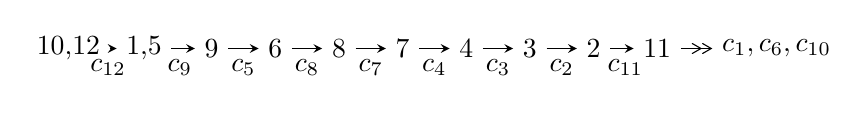
\begin{tikzpicture}[x=23pt, y=7pt]
	% node
	\node (A0) at (-1/8, 0) {10,12};
	\node (A1) at (17/16, 0) {1,5};
	\node (A2) at (17/8, 0) {9};
	\node (A3) at (25/8, 0) {6};
	\node (A4) at (33/8, 0) {8};
	\node (A5) at (41/8, 0) {7};
	\node (A6) at (49/8, 0) {4};
	\node (A7) at (57/8, 0) {3};
	\node (A8) at (65/8, 0) {2};
	\node (A9) at (73/8, 0) {11};
	\node (C1) at (1/2, -1) {$c_{12}$};
	\node (C2) at (13/8, -1) {$c_{9}$};
	\node (C3) at (21/8, -1) {$c_{5}$};
	\node (C4) at (29/8, -1) {$c_{8}$};
	\node (C5) at (37/8, -1) {$c_{7}$};
	\node (C6) at (45/8, -1) {$c_{4}$};
	\node (C7) at (53/8, -1) {$c_{3}$};
	\node (C8) at (61/8, -1) {$c_{2}$};
	\node (C9) at (69/8, -1) {$c_{11}$};
	\node (A10) at (11, 0) {$c_{1},c_{6},c_{10}$};

	% edge
	\draw[->,>=stealth]	
	(A0) edge (A1) (A1) edge (A2) (A2) edge (A3) (A3) edge (A4) (A4) edge (A5) (A5) edge (A6) (A6) edge (A7) (A7) edge (A8) (A8) edge (A9) ;
	\draw[->>,>={angle 60}]	
	(A9) edge (A10);
\end{tikzpicture} \\ 

\end{tabular} \\

\footnotetext{
The image of knot diagram is generated by the software ``\textbf{Draw programme}" developed by Andrew Bartholomew(\url{http://www.layer8.co.uk/maths/draw/index.htm\#Running-draw}), where we modified some parts for our purpose(\url{https://github.com/CATsTAILs/LinksPainter}).
}\phantom \\ \newline 
\centering \textbf{Ideals for irreducible components\footnotemark of $X_{\text{par}}$} 
 
\begin{align*}
I^u_{1}&=\langle 
1.31329\times10^{500} u^{97}+8.98067\times10^{500} u^{96}+\cdots+8.24393\times10^{497} b+8.17734\times10^{500},\\
\phantom{I^u_{1}}&\phantom{= \langle  }9.50553\times10^{500} u^{97}+6.50354\times10^{501} u^{96}+\cdots+8.24393\times10^{497} a+5.99735\times10^{501},\;u^{98}+7 u^{97}+\cdots+23 u+1\rangle \\
I^u_{2}&=\langle 
-6.44895\times10^{46} u^{35}+5.28645\times10^{47} u^{34}+\cdots+1.75776\times10^{44} b+1.79988\times10^{46},\\
\phantom{I^u_{2}}&\phantom{= \langle  }-2.46365\times10^{46} u^{35}+2.08684\times10^{47} u^{34}+\cdots+1.75776\times10^{44} a+5.21540\times10^{46},\\
\phantom{I^u_{2}}&\phantom{= \langle  }u^{36}-9 u^{35}+\cdots-14 u+1\rangle \\
I^u_{3}&=\langle 
- u^3+4 u^2+2 b-4 u-3,\;u^3-4 u^2+a+5 u,\;u^4-3 u^3+2 u^2+3 u+1\rangle \\
I^u_{4}&=\langle 
b^2- b+1,\;a,\;u-1\rangle \\
\\
\end{align*}
\raggedright * 4 irreducible components of $\dim_{\mathbb{C}}=0$, with total 140 representations.\\
\footnotetext{All coefficients of polynomials are rational numbers. But the coefficients are sometimes approximated in decimal forms when there is not enough margin.}
\newpage
\renewcommand{\arraystretch}{1}
\centering \section*{I. $I^u_{1}= \langle 1.31\times10^{500} u^{97}+8.98\times10^{500} u^{96}+\cdots+8.24\times10^{497} b+8.18\times10^{500},\;9.51\times10^{500} u^{97}+6.50\times10^{501} u^{96}+\cdots+8.24\times10^{497} a+6.00\times10^{501},\;u^{98}+7 u^{97}+\cdots+23 u+1 \rangle$}
\flushleft \textbf{(i) Arc colorings}\\
\begin{tabular}{m{7pt} m{180pt} m{7pt} m{180pt} }
\flushright $a_{10}=$&$\begin{pmatrix}0\\u\end{pmatrix}$ \\
\flushright $a_{12}=$&$\begin{pmatrix}1\\0\end{pmatrix}$ \\
\flushright $a_{1}=$&$\begin{pmatrix}1\\- u^2\end{pmatrix}$ \\
\flushright $a_{5}=$&$\begin{pmatrix}-1153.03 u^{97}-7888.88 u^{96}+\cdots-121463. u-7274.87\\-159.304 u^{97}-1089.37 u^{96}+\cdots-16618.9 u-991.922\end{pmatrix}$ \\
\flushright $a_{9}=$&$\begin{pmatrix}103.914 u^{97}+710.905 u^{96}+\cdots+10896.2 u+647.011\\-291.954 u^{97}-1997.45 u^{96}+\cdots-30797.8 u-1846.86\end{pmatrix}$ \\
\flushright $a_{6}=$&$\begin{pmatrix}-198.268 u^{97}-1356.61 u^{96}+\cdots-20919.8 u-1252.01\\29.8923 u^{97}+204.433 u^{96}+\cdots+3152.92 u+189.763\end{pmatrix}$ \\
\flushright $a_{8}=$&$\begin{pmatrix}395.868 u^{97}+2708.36 u^{96}+\cdots+41694.0 u+2493.87\\-291.954 u^{97}-1997.45 u^{96}+\cdots-30797.8 u-1846.86\end{pmatrix}$ \\
\flushright $a_{7}=$&$\begin{pmatrix}113.875 u^{97}+779.009 u^{96}+\cdots+11942.8 u+709.727\\-284.872 u^{97}-1949.02 u^{96}+\cdots-30054.1 u-1802.26\end{pmatrix}$ \\
\flushright $a_{4}=$&$\begin{pmatrix}-576.546 u^{97}-3943.09 u^{96}+\cdots-60413.0 u-3613.27\\59.4127 u^{97}+406.296 u^{96}+\cdots+6243.88 u+375.722\end{pmatrix}$ \\
\flushright $a_{3}=$&$\begin{pmatrix}-517.134 u^{97}-3536.80 u^{96}+\cdots-54169.1 u-3237.55\\59.4127 u^{97}+406.296 u^{96}+\cdots+6243.88 u+375.722\end{pmatrix}$ \\
\flushright $a_{2}=$&$\begin{pmatrix}-606.313 u^{97}-4147.30 u^{96}+\cdots-63505.5 u-3796.33\\124.345 u^{97}+850.757 u^{96}+\cdots+13140.3 u+789.560\end{pmatrix}$ \\
\flushright $a_{11}=$&$\begin{pmatrix}535.816 u^{97}+3668.17 u^{96}+\cdots+56813.0 u+3403.58\\-136.440 u^{97}-933.779 u^{96}+\cdots-14503.0 u-872.106\end{pmatrix}$\\&\end{tabular}
\flushleft \textbf{(ii) Obstruction class $= -1$}\\~\\
\flushleft \textbf{(iii) Cusp Shapes $= -468.986 u^{97}-3203.64 u^{96}+\cdots-48507.0 u-2901.05$}\\~\\
\newpage\renewcommand{\arraystretch}{1}
\flushleft \textbf{(iv) u-Polynomials at the component}\newline \\
\begin{tabular}{m{50pt}|m{274pt}}
Crossings & \hspace{64pt}u-Polynomials at each crossing \\
\hline $$\begin{aligned}c_{1}\end{aligned}$$&$\begin{aligned}
&u^{98}-7 u^{97}+\cdots-25602 u+2657
\end{aligned}$\\
\hline $$\begin{aligned}c_{2},c_{6}\end{aligned}$$&$\begin{aligned}
&u^{98}-3 u^{97}+\cdots-216906 u+13157
\end{aligned}$\\
\hline $$\begin{aligned}c_{3},c_{11}\end{aligned}$$&$\begin{aligned}
&u^{98}+2 u^{97}+\cdots+26608 u+508
\end{aligned}$\\
\hline $$\begin{aligned}c_{4}\end{aligned}$$&$\begin{aligned}
&u^{98}-5 u^{97}+\cdots-433 u+23
\end{aligned}$\\
\hline $$\begin{aligned}c_{5},c_{9}\end{aligned}$$&$\begin{aligned}
&u^{98}+42 u^{96}+\cdots+140656 u+34228
\end{aligned}$\\
\hline $$\begin{aligned}c_{7}\end{aligned}$$&$\begin{aligned}
&u^{98}-7 u^{97}+\cdots-2048 u+64
\end{aligned}$\\
\hline $$\begin{aligned}c_{8}\end{aligned}$$&$\begin{aligned}
&u^{98}+20 u^{96}+\cdots-26534568 u+43283857
\end{aligned}$\\
\hline $$\begin{aligned}c_{10}\end{aligned}$$&$\begin{aligned}
&u^{98}+12 u^{97}+\cdots-2720881 u+1109443
\end{aligned}$\\
\hline $$\begin{aligned}c_{12}\end{aligned}$$&$\begin{aligned}
&u^{98}+7 u^{97}+\cdots+23 u+1
\end{aligned}$\\
\hline
\end{tabular}\\~\\
\newpage\renewcommand{\arraystretch}{1}
\flushleft \textbf{(v) Riley Polynomials at the component}\newline \\
\begin{tabular}{m{50pt}|m{274pt}}
Crossings & \hspace{64pt}Riley Polynomials at each crossing \\
\hline $$\begin{aligned}c_{1}\end{aligned}$$&$\begin{aligned}
&y^{98}-55 y^{97}+\cdots-751130346 y+7059649
\end{aligned}$\\
\hline $$\begin{aligned}c_{2},c_{6}\end{aligned}$$&$\begin{aligned}
&y^{98}+103 y^{97}+\cdots-27972220618 y+173106649
\end{aligned}$\\
\hline $$\begin{aligned}c_{3},c_{11}\end{aligned}$$&$\begin{aligned}
&y^{98}-94 y^{97}+\cdots+1054871872 y+258064
\end{aligned}$\\
\hline $$\begin{aligned}c_{4}\end{aligned}$$&$\begin{aligned}
&y^{98}+9 y^{97}+\cdots-26167 y+529
\end{aligned}$\\
\hline $$\begin{aligned}c_{5},c_{9}\end{aligned}$$&$\begin{aligned}
&y^{98}+84 y^{97}+\cdots+44846020736 y+1171555984
\end{aligned}$\\
\hline $$\begin{aligned}c_{7}\end{aligned}$$&$\begin{aligned}
&y^{98}-3 y^{97}+\cdots-30720 y+4096
\end{aligned}$\\
\hline $$\begin{aligned}c_{8}\end{aligned}$$&$\begin{aligned}
&y^{98}+40 y^{97}+\cdots+141207617788579830 y+1873492276796449
\end{aligned}$\\
\hline $$\begin{aligned}c_{10}\end{aligned}$$&$\begin{aligned}
&y^{98}+36 y^{97}+\cdots+14973133605321 y+1230863770249
\end{aligned}$\\
\hline $$\begin{aligned}c_{12}\end{aligned}$$&$\begin{aligned}
&y^{98}-21 y^{97}+\cdots-79 y+1
\end{aligned}$\\
\hline
\end{tabular}\\~\\
\newpage\flushleft \textbf{(vi) Complex Volumes and Cusp Shapes}
$$\begin{array}{c|c|c}  
\text{Solutions to }I^u_{1}& \I (\text{vol} + \sqrt{-1}CS) & \text{Cusp shape}\\
 \hline 
\begin{aligned}
u &= \phantom{-}0.297779 + 0.962394 I \\
a &= \phantom{-}1.022180 + 0.169332 I \\
b &= \phantom{-}1.58919 - 0.84969 I\end{aligned}
 & -2.44786 + 2.28046 I & \phantom{-0.000000 } 0 \\ \hline\begin{aligned}
u &= \phantom{-}0.297779 - 0.962394 I \\
a &= \phantom{-}1.022180 - 0.169332 I \\
b &= \phantom{-}1.58919 + 0.84969 I\end{aligned}
 & -2.44786 - 2.28046 I & \phantom{-0.000000 } 0 \\ \hline\begin{aligned}
u &= \phantom{-}1.010880 + 0.161137 I \\
a &= -0.213420 - 1.269340 I \\
b &= -0.21564 - 1.61424 I\end{aligned}
 & -7.52661 + 5.04383 I & \phantom{-0.000000 } 0 \\ \hline\begin{aligned}
u &= \phantom{-}1.010880 - 0.161137 I \\
a &= -0.213420 + 1.269340 I \\
b &= -0.21564 + 1.61424 I\end{aligned}
 & -7.52661 - 5.04383 I & \phantom{-0.000000 } 0 \\ \hline\begin{aligned}
u &= -0.621792 + 0.819445 I \\
a &= \phantom{-}0.582418 + 0.765895 I \\
b &= \phantom{-}0.344815 + 0.764548 I\end{aligned}
 & -8.25028 - 2.12975 I & \phantom{-0.000000 } 0 \\ \hline\begin{aligned}
u &= -0.621792 - 0.819445 I \\
a &= \phantom{-}0.582418 - 0.765895 I \\
b &= \phantom{-}0.344815 - 0.764548 I\end{aligned}
 & -8.25028 + 2.12975 I & \phantom{-0.000000 } 0 \\ \hline\begin{aligned}
u &= -0.896403 + 0.592844 I \\
a &= \phantom{-}0.966816 + 0.375746 I \\
b &= \phantom{-}0.199042 + 0.683208 I\end{aligned}
 & -7.20927 - 3.04632 I & \phantom{-0.000000 } 0 \\ \hline\begin{aligned}
u &= -0.896403 - 0.592844 I \\
a &= \phantom{-}0.966816 - 0.375746 I \\
b &= \phantom{-}0.199042 - 0.683208 I\end{aligned}
 & -7.20927 + 3.04632 I & \phantom{-0.000000 } 0 \\ \hline\begin{aligned}
u &= \phantom{-}0.875671 + 0.627105 I \\
a &= \phantom{-}0.247782 + 0.053577 I \\
b &= \phantom{-}0.979738 + 0.820171 I\end{aligned}
 & -0.46733 + 5.54468 I & \phantom{-0.000000 } 0 \\ \hline\begin{aligned}
u &= \phantom{-}0.875671 - 0.627105 I \\
a &= \phantom{-}0.247782 - 0.053577 I \\
b &= \phantom{-}0.979738 - 0.820171 I\end{aligned}
 & -0.46733 - 5.54468 I & \phantom{-0.000000 } 0\\
 \hline 
 \end{array}$$\newpage$$\begin{array}{c|c|c}  
\text{Solutions to }I^u_{1}& \I (\text{vol} + \sqrt{-1}CS) & \text{Cusp shape}\\
 \hline 
\begin{aligned}
u &= -0.915061 + 0.054031 I \\
a &= -0.273898 - 0.828206 I \\
b &= \phantom{-}0.034152 - 1.395890 I\end{aligned}
 & \phantom{-}3.75773 + 1.09085 I & \phantom{-0.000000 } 0 \\ \hline\begin{aligned}
u &= -0.915061 - 0.054031 I \\
a &= -0.273898 + 0.828206 I \\
b &= \phantom{-}0.034152 + 1.395890 I\end{aligned}
 & \phantom{-}3.75773 - 1.09085 I & \phantom{-0.000000 } 0 \\ \hline\begin{aligned}
u &= \phantom{-}0.876386 + 0.637072 I \\
a &= \phantom{-}0.965490 + 0.211185 I \\
b &= \phantom{-}1.312150 - 0.279787 I\end{aligned}
 & \phantom{-}0.32102 + 5.18997 I & \phantom{-0.000000 } 0 \\ \hline\begin{aligned}
u &= \phantom{-}0.876386 - 0.637072 I \\
a &= \phantom{-}0.965490 - 0.211185 I \\
b &= \phantom{-}1.312150 + 0.279787 I\end{aligned}
 & \phantom{-}0.32102 - 5.18997 I & \phantom{-0.000000 } 0 \\ \hline\begin{aligned}
u &= -0.792067 + 0.364533 I \\
a &= \phantom{-}1.064860 - 0.751526 I \\
b &= \phantom{-}0.849227 - 0.435183 I\end{aligned}
 & -1.46403 - 8.46772 I & \phantom{-0.000000 } 0 \\ \hline\begin{aligned}
u &= -0.792067 - 0.364533 I \\
a &= \phantom{-}1.064860 + 0.751526 I \\
b &= \phantom{-}0.849227 + 0.435183 I\end{aligned}
 & -1.46403 + 8.46772 I & \phantom{-0.000000 } 0 \\ \hline\begin{aligned}
u &= -0.672626 + 0.905633 I \\
a &= \phantom{-}1.222900 - 0.347747 I \\
b &= \phantom{-}2.49118 + 0.26599 I\end{aligned}
 & -12.4233 - 7.4999 I & \phantom{-0.000000 } 0 \\ \hline\begin{aligned}
u &= -0.672626 - 0.905633 I \\
a &= \phantom{-}1.222900 + 0.347747 I \\
b &= \phantom{-}2.49118 - 0.26599 I\end{aligned}
 & -12.4233 + 7.4999 I & \phantom{-0.000000 } 0 \\ \hline\begin{aligned}
u &= -0.502964 + 0.672687 I \\
a &= -0.112785 + 0.315563 I \\
b &= \phantom{-}0.638997 + 0.143982 I\end{aligned}
 & -2.47697 + 1.40445 I & \phantom{-0.000000 } 0 \\ \hline\begin{aligned}
u &= -0.502964 - 0.672687 I \\
a &= -0.112785 - 0.315563 I \\
b &= \phantom{-}0.638997 - 0.143982 I\end{aligned}
 & -2.47697 - 1.40445 I & \phantom{-0.000000 } 0\\
 \hline 
 \end{array}$$\newpage$$\begin{array}{c|c|c}  
\text{Solutions to }I^u_{1}& \I (\text{vol} + \sqrt{-1}CS) & \text{Cusp shape}\\
 \hline 
\begin{aligned}
u &= -0.902378 + 0.740032 I \\
a &= -0.476203 + 1.088780 I \\
b &= -1.62606 - 0.36286 I\end{aligned}
 & -12.39800 + 2.77753 I & \phantom{-0.000000 } 0 \\ \hline\begin{aligned}
u &= -0.902378 - 0.740032 I \\
a &= -0.476203 - 1.088780 I \\
b &= -1.62606 + 0.36286 I\end{aligned}
 & -12.39800 - 2.77753 I & \phantom{-0.000000 } 0 \\ \hline\begin{aligned}
u &= -0.719806 + 0.334419 I \\
a &= \phantom{-}0.839821 - 0.983498 I \\
b &= \phantom{-}0.857987 - 0.394289 I\end{aligned}
 & -3.32757 - 0.74133 I & \phantom{-0.000000 } 0 \\ \hline\begin{aligned}
u &= -0.719806 - 0.334419 I \\
a &= \phantom{-}0.839821 + 0.983498 I \\
b &= \phantom{-}0.857987 + 0.394289 I\end{aligned}
 & -3.32757 + 0.74133 I & \phantom{-0.000000 } 0 \\ \hline\begin{aligned}
u &= \phantom{-}0.815536 + 0.923671 I \\
a &= \phantom{-}0.211361 - 0.892570 I \\
b &= -0.292264 + 0.219911 I\end{aligned}
 & \phantom{-}0.147768 + 0.601523 I & \phantom{-0.000000 } 0 \\ \hline\begin{aligned}
u &= \phantom{-}0.815536 - 0.923671 I \\
a &= \phantom{-}0.211361 + 0.892570 I \\
b &= -0.292264 - 0.219911 I\end{aligned}
 & \phantom{-}0.147768 - 0.601523 I & \phantom{-0.000000 } 0 \\ \hline\begin{aligned}
u &= -0.993894 + 0.739046 I \\
a &= \phantom{-}0.372429 + 0.295295 I \\
b &= \phantom{-}0.168599 - 0.122446 I\end{aligned}
 & -1.37363 - 6.86287 I & \phantom{-0.000000 } 0 \\ \hline\begin{aligned}
u &= -0.993894 - 0.739046 I \\
a &= \phantom{-}0.372429 - 0.295295 I \\
b &= \phantom{-}0.168599 + 0.122446 I\end{aligned}
 & -1.37363 + 6.86287 I & \phantom{-0.000000 } 0 \\ \hline\begin{aligned}
u &= \phantom{-}0.344938 + 0.638925 I \\
a &= \phantom{-}0.274724 + 0.765846 I \\
b &= \phantom{-}0.163839 - 0.856175 I\end{aligned}
 & -0.21248 + 1.79826 I & \phantom{-0.000000 } 0 \\ \hline\begin{aligned}
u &= \phantom{-}0.344938 - 0.638925 I \\
a &= \phantom{-}0.274724 - 0.765846 I \\
b &= \phantom{-}0.163839 + 0.856175 I\end{aligned}
 & -0.21248 - 1.79826 I & \phantom{-0.000000 } 0\\
 \hline 
 \end{array}$$\newpage$$\begin{array}{c|c|c}  
\text{Solutions to }I^u_{1}& \I (\text{vol} + \sqrt{-1}CS) & \text{Cusp shape}\\
 \hline 
\begin{aligned}
u &= \phantom{-}0.374511 + 1.218040 I \\
a &= -1.127910 - 0.152756 I \\
b &= -1.63102 + 0.44266 I\end{aligned}
 & -5.94774 + 6.35238 I & \phantom{-0.000000 } 0 \\ \hline\begin{aligned}
u &= \phantom{-}0.374511 - 1.218040 I \\
a &= -1.127910 + 0.152756 I \\
b &= -1.63102 - 0.44266 I\end{aligned}
 & -5.94774 - 6.35238 I & \phantom{-0.000000 } 0 \\ \hline\begin{aligned}
u &= \phantom{-}0.664993 + 1.095230 I \\
a &= -1.046210 - 0.547420 I \\
b &= -1.88449 + 0.56737 I\end{aligned}
 & -8.39095 - 0.53811 I & \phantom{-0.000000 } 0 \\ \hline\begin{aligned}
u &= \phantom{-}0.664993 - 1.095230 I \\
a &= -1.046210 + 0.547420 I \\
b &= -1.88449 - 0.56737 I\end{aligned}
 & -8.39095 + 0.53811 I & \phantom{-0.000000 } 0 \\ \hline\begin{aligned}
u &= -0.936379 + 0.874958 I \\
a &= \phantom{-}1.094090 - 0.548079 I \\
b &= \phantom{-}2.20657 + 0.71506 I\end{aligned}
 & -12.4049 - 8.9977 I & \phantom{-0.000000 } 0 \\ \hline\begin{aligned}
u &= -0.936379 - 0.874958 I \\
a &= \phantom{-}1.094090 + 0.548079 I \\
b &= \phantom{-}2.20657 - 0.71506 I\end{aligned}
 & -12.4049 + 8.9977 I & \phantom{-0.000000 } 0 \\ \hline\begin{aligned}
u &= -0.744621 + 1.043820 I \\
a &= -1.022590 + 0.676287 I \\
b &= -1.68981 - 0.63987 I\end{aligned}
 & -7.71494 - 4.90990 I & \phantom{-0.000000 } 0 \\ \hline\begin{aligned}
u &= -0.744621 - 1.043820 I \\
a &= -1.022590 - 0.676287 I \\
b &= -1.68981 + 0.63987 I\end{aligned}
 & -7.71494 + 4.90990 I & \phantom{-0.000000 } 0 \\ \hline\begin{aligned}
u &= -1.175390 + 0.516378 I \\
a &= -0.622936 - 0.849858 I \\
b &= -1.34008 - 0.54188 I\end{aligned}
 & -6.12476 + 3.89475 I & \phantom{-0.000000 } 0 \\ \hline\begin{aligned}
u &= -1.175390 - 0.516378 I \\
a &= -0.622936 + 0.849858 I \\
b &= -1.34008 + 0.54188 I\end{aligned}
 & -6.12476 - 3.89475 I & \phantom{-0.000000 } 0\\
 \hline 
 \end{array}$$\newpage$$\begin{array}{c|c|c}  
\text{Solutions to }I^u_{1}& \I (\text{vol} + \sqrt{-1}CS) & \text{Cusp shape}\\
 \hline 
\begin{aligned}
u &= -0.328261 + 1.249000 I \\
a &= \phantom{-}1.25659 - 0.83325 I \\
b &= \phantom{-}1.299970 + 0.167085 I\end{aligned}
 & -13.11780 - 1.97601 I & \phantom{-0.000000 } 0 \\ \hline\begin{aligned}
u &= -0.328261 - 1.249000 I \\
a &= \phantom{-}1.25659 + 0.83325 I \\
b &= \phantom{-}1.299970 - 0.167085 I\end{aligned}
 & -13.11780 + 1.97601 I & \phantom{-0.000000 } 0 \\ \hline\begin{aligned}
u &= -0.601045 + 0.319523 I \\
a &= -1.47869 + 0.84409 I \\
b &= -1.006790 + 0.230868 I\end{aligned}
 & \phantom{-}0.46988 - 3.49771 I & \phantom{-0.000000 } 0 \\ \hline\begin{aligned}
u &= -0.601045 - 0.319523 I \\
a &= -1.47869 - 0.84409 I \\
b &= -1.006790 - 0.230868 I\end{aligned}
 & \phantom{-}0.46988 + 3.49771 I & \phantom{-0.000000 } 0 \\ \hline\begin{aligned}
u &= \phantom{-}0.678764 + 0.023481 I \\
a &= \phantom{-}1.165110 + 0.262883 I \\
b &= -0.202309 + 0.037094 I\end{aligned}
 & \phantom{-}1.49876 + 0.09907 I & \phantom{-0.000000 } 0 \\ \hline\begin{aligned}
u &= \phantom{-}0.678764 - 0.023481 I \\
a &= \phantom{-}1.165110 - 0.262883 I \\
b &= -0.202309 - 0.037094 I\end{aligned}
 & \phantom{-}1.49876 - 0.09907 I & \phantom{-0.000000 } 0 \\ \hline\begin{aligned}
u &= -0.202651 + 0.646746 I \\
a &= \phantom{-}0.504766 + 1.251150 I \\
b &= \phantom{-}0.402736 - 0.412523 I\end{aligned}
 & -0.38569 + 2.12879 I & \phantom{-0.000000 } 0 \\ \hline\begin{aligned}
u &= -0.202651 - 0.646746 I \\
a &= \phantom{-}0.504766 - 1.251150 I \\
b &= \phantom{-}0.402736 + 0.412523 I\end{aligned}
 & -0.38569 - 2.12879 I & \phantom{-0.000000 } 0 \\ \hline\begin{aligned}
u &= -0.863600 + 1.019240 I \\
a &= -0.767920 - 0.879189 I \\
b &= -0.346321 - 0.321968 I\end{aligned}
 & -7.46331 - 10.46160 I & \phantom{-0.000000 } 0 \\ \hline\begin{aligned}
u &= -0.863600 - 1.019240 I \\
a &= -0.767920 + 0.879189 I \\
b &= -0.346321 + 0.321968 I\end{aligned}
 & -7.46331 + 10.46160 I & \phantom{-0.000000 } 0\\
 \hline 
 \end{array}$$\newpage$$\begin{array}{c|c|c}  
\text{Solutions to }I^u_{1}& \I (\text{vol} + \sqrt{-1}CS) & \text{Cusp shape}\\
 \hline 
\begin{aligned}
u &= \phantom{-}1.217230 + 0.669504 I \\
a &= -0.112972 + 0.543057 I \\
b &= -0.167988 - 0.464929 I\end{aligned}
 & \phantom{-}2.32202 + 2.06905 I & \phantom{-0.000000 } 0 \\ \hline\begin{aligned}
u &= \phantom{-}1.217230 - 0.669504 I \\
a &= -0.112972 - 0.543057 I \\
b &= -0.167988 + 0.464929 I\end{aligned}
 & \phantom{-}2.32202 - 2.06905 I & \phantom{-0.000000 } 0 \\ \hline\begin{aligned}
u &= \phantom{-}0.557808 + 0.223218 I \\
a &= \phantom{-}1.03702 + 1.07809 I \\
b &= \phantom{-}0.56620 + 1.88391 I\end{aligned}
 & -2.54420 + 3.14291 I & \phantom{-}2.00000 - 10.38283 I \\ \hline\begin{aligned}
u &= \phantom{-}0.557808 - 0.223218 I \\
a &= \phantom{-}1.03702 - 1.07809 I \\
b &= \phantom{-}0.56620 - 1.88391 I\end{aligned}
 & -2.54420 - 3.14291 I & \phantom{-}2.00000 + 10.38283 I \\ \hline\begin{aligned}
u &= \phantom{-}1.304760 + 0.530697 I \\
a &= \phantom{-}0.136175 - 0.830160 I \\
b &= -0.0066614 + 0.0625832 I\end{aligned}
 & \phantom{-}0.489098 + 0.388700 I & \phantom{-0.000000 } 0 \\ \hline\begin{aligned}
u &= \phantom{-}1.304760 - 0.530697 I \\
a &= \phantom{-}0.136175 + 0.830160 I \\
b &= -0.0066614 - 0.0625832 I\end{aligned}
 & \phantom{-}0.489098 - 0.388700 I & \phantom{-0.000000 } 0 \\ \hline\begin{aligned}
u &= \phantom{-}0.376700 + 0.454340 I \\
a &= -3.06674 - 1.14555 I \\
b &= -0.932034 + 0.551422 I\end{aligned}
 & -10.42540 + 6.06568 I & -1.8335 - 15.3637 I \\ \hline\begin{aligned}
u &= \phantom{-}0.376700 - 0.454340 I \\
a &= -3.06674 + 1.14555 I \\
b &= -0.932034 - 0.551422 I\end{aligned}
 & -10.42540 - 6.06568 I & -1.8335 + 15.3637 I \\ \hline\begin{aligned}
u &= \phantom{-}0.554881 + 0.140141 I \\
a &= \phantom{-}0.27046 + 1.79547 I \\
b &= \phantom{-}0.453971 - 0.844268 I\end{aligned}
 & -0.06150 + 2.48943 I & \phantom{-}3.17370 - 4.01834 I \\ \hline\begin{aligned}
u &= \phantom{-}0.554881 - 0.140141 I \\
a &= \phantom{-}0.27046 - 1.79547 I \\
b &= \phantom{-}0.453971 + 0.844268 I\end{aligned}
 & -0.06150 - 2.48943 I & \phantom{-}3.17370 + 4.01834 I\\
 \hline 
 \end{array}$$\newpage$$\begin{array}{c|c|c}  
\text{Solutions to }I^u_{1}& \I (\text{vol} + \sqrt{-1}CS) & \text{Cusp shape}\\
 \hline 
\begin{aligned}
u &= \phantom{-}1.19386 + 0.86245 I \\
a &= -0.501291 - 0.565693 I \\
b &= -1.50989 + 0.01628 I\end{aligned}
 & -1.87185 + 3.47822 I & \phantom{-0.000000 } 0 \\ \hline\begin{aligned}
u &= \phantom{-}1.19386 - 0.86245 I \\
a &= -0.501291 + 0.565693 I \\
b &= -1.50989 - 0.01628 I\end{aligned}
 & -1.87185 - 3.47822 I & \phantom{-0.000000 } 0 \\ \hline\begin{aligned}
u &= \phantom{-}1.24300 + 0.89145 I \\
a &= \phantom{-}0.681143 + 0.699008 I \\
b &= \phantom{-}1.98865 - 0.52084 I\end{aligned}
 & -6.59645 + 7.81675 I & \phantom{-0.000000 } 0 \\ \hline\begin{aligned}
u &= \phantom{-}1.24300 - 0.89145 I \\
a &= \phantom{-}0.681143 - 0.699008 I \\
b &= \phantom{-}1.98865 + 0.52084 I\end{aligned}
 & -6.59645 - 7.81675 I & \phantom{-0.000000 } 0 \\ \hline\begin{aligned}
u &= -0.099402 + 0.428459 I \\
a &= -2.36898 + 2.26274 I \\
b &= -1.39345 - 0.42785 I\end{aligned}
 & -11.61500 + 2.97623 I & -4.67472 - 1.54835 I \\ \hline\begin{aligned}
u &= -0.099402 - 0.428459 I \\
a &= -2.36898 - 2.26274 I \\
b &= -1.39345 + 0.42785 I\end{aligned}
 & -11.61500 - 2.97623 I & -4.67472 + 1.54835 I \\ \hline\begin{aligned}
u &= -0.416159 + 0.139948 I \\
a &= -2.18643 + 1.00702 I \\
b &= -0.590900 + 0.023581 I\end{aligned}
 & \phantom{-}1.41101 - 1.64765 I & \phantom{-}4.38403 + 7.71230 I \\ \hline\begin{aligned}
u &= -0.416159 - 0.139948 I \\
a &= -2.18643 - 1.00702 I \\
b &= -0.590900 - 0.023581 I\end{aligned}
 & \phantom{-}1.41101 + 1.64765 I & \phantom{-}4.38403 - 7.71230 I \\ \hline\begin{aligned}
u &= -1.27052 + 0.92169 I \\
a &= \phantom{-}0.688840 - 0.639863 I \\
b &= \phantom{-}1.87760 + 0.38054 I\end{aligned}
 & -6.07607 - 2.31012 I & \phantom{-0.000000 } 0 \\ \hline\begin{aligned}
u &= -1.27052 - 0.92169 I \\
a &= \phantom{-}0.688840 + 0.639863 I \\
b &= \phantom{-}1.87760 - 0.38054 I\end{aligned}
 & -6.07607 + 2.31012 I & \phantom{-0.000000 } 0\\
 \hline 
 \end{array}$$\newpage$$\begin{array}{c|c|c}  
\text{Solutions to }I^u_{1}& \I (\text{vol} + \sqrt{-1}CS) & \text{Cusp shape}\\
 \hline 
\begin{aligned}
u &= -0.367068 + 0.160217 I \\
a &= -2.60294 + 2.27563 I \\
b &= -0.617257 - 0.732831 I\end{aligned}
 & \phantom{-}1.75773 - 1.88898 I & \phantom{-}19.6084 - 9.7659 I \\ \hline\begin{aligned}
u &= -0.367068 - 0.160217 I \\
a &= -2.60294 - 2.27563 I \\
b &= -0.617257 + 0.732831 I\end{aligned}
 & \phantom{-}1.75773 + 1.88898 I & \phantom{-}19.6084 + 9.7659 I \\ \hline\begin{aligned}
u &= -1.20084 + 1.07188 I \\
a &= -0.946736 + 0.444946 I \\
b &= -2.20732 - 0.57872 I\end{aligned}
 & -12.4887 - 18.1031 I & \phantom{-0.000000 } 0 \\ \hline\begin{aligned}
u &= -1.20084 - 1.07188 I \\
a &= -0.946736 - 0.444946 I \\
b &= -2.20732 + 0.57872 I\end{aligned}
 & -12.4887 + 18.1031 I & \phantom{-0.000000 } 0 \\ \hline\begin{aligned}
u &= \phantom{-}1.16072 + 1.12461 I \\
a &= -0.742562 - 0.133966 I \\
b &= -2.28470 + 0.61290 I\end{aligned}
 & \phantom{-}1.57710 + 7.14701 I & \phantom{-0.000000 } 0 \\ \hline\begin{aligned}
u &= \phantom{-}1.16072 - 1.12461 I \\
a &= -0.742562 + 0.133966 I \\
b &= -2.28470 - 0.61290 I\end{aligned}
 & \phantom{-}1.57710 - 7.14701 I & \phantom{-0.000000 } 0 \\ \hline\begin{aligned}
u &= -1.19450 + 1.10023 I \\
a &= \phantom{-}0.712857 - 0.499549 I \\
b &= \phantom{-}2.11446 + 0.79329 I\end{aligned}
 & -5.99457 - 10.31610 I & \phantom{-0.000000 } 0 \\ \hline\begin{aligned}
u &= -1.19450 - 1.10023 I \\
a &= \phantom{-}0.712857 + 0.499549 I \\
b &= \phantom{-}2.11446 - 0.79329 I\end{aligned}
 & -5.99457 + 10.31610 I & \phantom{-0.000000 } 0 \\ \hline\begin{aligned}
u &= \phantom{-}0.191209 + 0.306647 I \\
a &= \phantom{-}1.43023 + 0.62187 I \\
b &= -0.30448 - 3.78683 I\end{aligned}
 & -4.46447 + 5.23065 I & -15.8390 + 3.5168 I \\ \hline\begin{aligned}
u &= \phantom{-}0.191209 - 0.306647 I \\
a &= \phantom{-}1.43023 - 0.62187 I \\
b &= -0.30448 + 3.78683 I\end{aligned}
 & -4.46447 - 5.23065 I & -15.8390 - 3.5168 I\\
 \hline 
 \end{array}$$\newpage$$\begin{array}{c|c|c}  
\text{Solutions to }I^u_{1}& \I (\text{vol} + \sqrt{-1}CS) & \text{Cusp shape}\\
 \hline 
\begin{aligned}
u &= -0.90440 + 1.40261 I \\
a &= -0.661781 + 0.425974 I \\
b &= -2.11701 - 0.67980 I\end{aligned}
 & -6.96776 + 1.62024 I & \phantom{-0.000000 } 0 \\ \hline\begin{aligned}
u &= -0.90440 - 1.40261 I \\
a &= -0.661781 - 0.425974 I \\
b &= -2.11701 + 0.67980 I\end{aligned}
 & -6.96776 - 1.62024 I & \phantom{-0.000000 } 0 \\ \hline\begin{aligned}
u &= \phantom{-}1.04890 + 1.34938 I \\
a &= \phantom{-}0.698921 + 0.255621 I \\
b &= \phantom{-}1.92274 - 0.86568 I\end{aligned}
 & -2.66284 + 5.40803 I & \phantom{-0.000000 } 0 \\ \hline\begin{aligned}
u &= \phantom{-}1.04890 - 1.34938 I \\
a &= \phantom{-}0.698921 - 0.255621 I \\
b &= \phantom{-}1.92274 + 0.86568 I\end{aligned}
 & -2.66284 - 5.40803 I & \phantom{-0.000000 } 0 \\ \hline\begin{aligned}
u &= -1.03230 + 1.39080 I \\
a &= \phantom{-}0.601176 - 0.727613 I \\
b &= \phantom{-}1.59571 + 0.41095 I\end{aligned}
 & -13.3115 + 9.4190 I & \phantom{-0.000000 } 0 \\ \hline\begin{aligned}
u &= -1.03230 - 1.39080 I \\
a &= \phantom{-}0.601176 + 0.727613 I \\
b &= \phantom{-}1.59571 - 0.41095 I\end{aligned}
 & -13.3115 - 9.4190 I & \phantom{-0.000000 } 0 \\ \hline\begin{aligned}
u &= -0.117543 + 0.220736 I \\
a &= -0.98093 + 4.64440 I \\
b &= \phantom{-}0.282949 - 0.016428 I\end{aligned}
 & -0.48485 - 2.96998 I & -5.78061 - 2.76336 I \\ \hline\begin{aligned}
u &= -0.117543 - 0.220736 I \\
a &= -0.98093 - 4.64440 I \\
b &= \phantom{-}0.282949 + 0.016428 I\end{aligned}
 & -0.48485 + 2.96998 I & -5.78061 + 2.76336 I \\ \hline\begin{aligned}
u &= \phantom{-}1.75469 + 0.35098 I \\
a &= -0.078590 - 0.419650 I \\
b &= -0.97885 + 1.47115 I\end{aligned}
 & \phantom{-}3.11758 + 3.82652 I & \phantom{-0.000000 } 0 \\ \hline\begin{aligned}
u &= \phantom{-}1.75469 - 0.35098 I \\
a &= -0.078590 + 0.419650 I \\
b &= -0.97885 - 1.47115 I\end{aligned}
 & \phantom{-}3.11758 - 3.82652 I & \phantom{-0.000000 } 0\\
 \hline 
 \end{array}$$\newpage$$\begin{array}{c|c|c}  
\text{Solutions to }I^u_{1}& \I (\text{vol} + \sqrt{-1}CS) & \text{Cusp shape}\\
 \hline 
\begin{aligned}
u &= -0.158595 + 0.000579 I \\
a &= -0.27132 - 5.75775 I \\
b &= \phantom{-}1.64593 - 0.78163 I\end{aligned}
 & -2.70884 - 1.02332 I & \phantom{-}1.77227 - 2.30546 I \\ \hline\begin{aligned}
u &= -0.158595 - 0.000579 I \\
a &= -0.27132 + 5.75775 I \\
b &= \phantom{-}1.64593 + 0.78163 I\end{aligned}
 & -2.70884 + 1.02332 I & \phantom{-}1.77227 + 2.30546 I \\ \hline\begin{aligned}
u &= -1.40148 + 1.37678 I \\
a &= -0.884947 + 0.442312 I \\
b &= -1.91337 - 0.27619 I\end{aligned}
 & -8.74306 - 7.50542 I & \phantom{-0.000000 } 0 \\ \hline\begin{aligned}
u &= -1.40148 - 1.37678 I \\
a &= -0.884947 - 0.442312 I \\
b &= -1.91337 + 0.27619 I\end{aligned}
 & -8.74306 + 7.50542 I & \phantom{-0.000000 } 0 \\ \hline\begin{aligned}
u &= -1.87585 + 0.68624 I \\
a &= -0.099794 + 0.580457 I \\
b &= -1.19365 - 1.50047 I\end{aligned}
 & -9.37416 + 1.26969 I & \phantom{-0.000000 } 0 \\ \hline\begin{aligned}
u &= -1.87585 - 0.68624 I \\
a &= -0.099794 - 0.580457 I \\
b &= -1.19365 + 1.50047 I\end{aligned}
 & -9.37416 - 1.26969 I & \phantom{-0.000000 } 0 \\ \hline\begin{aligned}
u &= \phantom{-}1.86439 + 1.30631 I \\
a &= \phantom{-}0.100434 + 0.639423 I \\
b &= \phantom{-}0.465943 - 0.834397 I\end{aligned}
 & \phantom{-}1.74223 + 2.15763 I & \phantom{-0.000000 } 0 \\ \hline\begin{aligned}
u &= \phantom{-}1.86439 - 1.30631 I \\
a &= \phantom{-}0.100434 - 0.639423 I \\
b &= \phantom{-}0.465943 + 0.834397 I\end{aligned}
 & \phantom{-}1.74223 - 2.15763 I & \phantom{-0.000000 } 0\\
 \hline 
 \end{array}$$\newpage\newpage\renewcommand{\arraystretch}{1}
\centering \section*{II. $I^u_{2}= \langle -6.45\times10^{46} u^{35}+5.29\times10^{47} u^{34}+\cdots+1.76\times10^{44} b+1.80\times10^{46},\;-2.46\times10^{46} u^{35}+2.09\times10^{47} u^{34}+\cdots+1.76\times10^{44} a+5.22\times10^{46},\;u^{36}-9 u^{35}+\cdots-14 u+1 \rangle$}
\flushleft \textbf{(i) Arc colorings}\\
\begin{tabular}{m{7pt} m{180pt} m{7pt} m{180pt} }
\flushright $a_{10}=$&$\begin{pmatrix}0\\u\end{pmatrix}$ \\
\flushright $a_{12}=$&$\begin{pmatrix}1\\0\end{pmatrix}$ \\
\flushright $a_{1}=$&$\begin{pmatrix}1\\- u^2\end{pmatrix}$ \\
\flushright $a_{5}=$&$\begin{pmatrix}140.158 u^{35}-1187.21 u^{34}+\cdots+3524.39 u-296.706\\366.884 u^{35}-3007.49 u^{34}+\cdots+2539.57 u-102.396\end{pmatrix}$ \\
\flushright $a_{9}=$&$\begin{pmatrix}238.295 u^{35}-1927.86 u^{34}+\cdots+1235.01 u-44.4770\\328.269 u^{35}-2833.09 u^{34}+\cdots+8330.09 u-666.273\end{pmatrix}$ \\
\flushright $a_{6}=$&$\begin{pmatrix}563.553 u^{35}-4811.95 u^{34}+\cdots+12684.8 u-991.409\\295.393 u^{35}-2429.91 u^{34}+\cdots+2251.27 u-98.4593\end{pmatrix}$ \\
\flushright $a_{8}=$&$\begin{pmatrix}-89.9730 u^{35}+905.235 u^{34}+\cdots-7095.08 u+621.796\\328.269 u^{35}-2833.09 u^{34}+\cdots+8330.09 u-666.273\end{pmatrix}$ \\
\flushright $a_{7}=$&$\begin{pmatrix}348.754 u^{35}-2849.01 u^{34}+\cdots+2661.67 u-139.954\\266.407 u^{35}-2283.23 u^{34}+\cdots+6048.60 u-471.972\end{pmatrix}$ \\
\flushright $a_{4}=$&$\begin{pmatrix}541.938 u^{35}-4736.15 u^{34}+\cdots+16865.3 u-1387.65\\-221.527 u^{35}+1946.78 u^{34}+\cdots-7346.51 u+620.328\end{pmatrix}$ \\
\flushright $a_{3}=$&$\begin{pmatrix}320.411 u^{35}-2789.37 u^{34}+\cdots+9518.75 u-767.324\\-221.527 u^{35}+1946.78 u^{34}+\cdots-7346.51 u+620.328\end{pmatrix}$ \\
\flushright $a_{2}=$&$\begin{pmatrix}647.693 u^{35}-5541.90 u^{34}+\cdots+13860.9 u-1062.14\\254.012 u^{35}-2185.29 u^{34}+\cdots+6133.90 u-488.778\end{pmatrix}$ \\
\flushright $a_{11}=$&$\begin{pmatrix}493.207 u^{35}-4306.08 u^{34}+\cdots+13158.1 u-1047.25\\-227.149 u^{35}+2008.25 u^{34}+\cdots-7499.57 u+621.554\end{pmatrix}$\\&\end{tabular}
\flushleft \textbf{(ii) Obstruction class $= 1$}\\~\\
\flushleft \textbf{(iii) Cusp Shapes $= 1583.96 u^{35}-13530.4 u^{34}+\cdots+35840.2 u-2796.67$}\\~\\
\newpage\renewcommand{\arraystretch}{1}
\flushleft \textbf{(iv) u-Polynomials at the component}\newline \\
\begin{tabular}{m{50pt}|m{274pt}}
Crossings & \hspace{64pt}u-Polynomials at each crossing \\
\hline $$\begin{aligned}c_{1}\end{aligned}$$&$\begin{aligned}
&u^{36}-14 u^{35}+\cdots-4 u+1
\end{aligned}$\\
\hline $$\begin{aligned}c_{2}\end{aligned}$$&$\begin{aligned}
&u^{36}-3 u^{35}+\cdots+9 u+1
\end{aligned}$\\
\hline $$\begin{aligned}c_{3}\end{aligned}$$&$\begin{aligned}
&u^{36}+u^{35}+\cdots+24 u+4
\end{aligned}$\\
\hline $$\begin{aligned}c_{4}\end{aligned}$$&$\begin{aligned}
&u^{36}-7 u^{35}+\cdots+23 u^2+1
\end{aligned}$\\
\hline $$\begin{aligned}c_{5}\end{aligned}$$&$\begin{aligned}
&u^{36}- u^{35}+\cdots+24 u+4
\end{aligned}$\\
\hline $$\begin{aligned}c_{6}\end{aligned}$$&$\begin{aligned}
&u^{36}+3 u^{35}+\cdots-9 u+1
\end{aligned}$\\
\hline $$\begin{aligned}c_{7}\end{aligned}$$&$\begin{aligned}
&u^{36}+2 u^{35}+\cdots+112 u+784
\end{aligned}$\\
\hline $$\begin{aligned}c_{8}\end{aligned}$$&$\begin{aligned}
&u^{36}- u^{35}+\cdots+98 u+13
\end{aligned}$\\
\hline $$\begin{aligned}c_{9}\end{aligned}$$&$\begin{aligned}
&u^{36}+u^{35}+\cdots-24 u+4
\end{aligned}$\\
\hline $$\begin{aligned}c_{10}\end{aligned}$$&$\begin{aligned}
&u^{36}+u^{34}+\cdots-2 u+1
\end{aligned}$\\
\hline $$\begin{aligned}c_{11}\end{aligned}$$&$\begin{aligned}
&u^{36}- u^{35}+\cdots-24 u+4
\end{aligned}$\\
\hline $$\begin{aligned}c_{12}\end{aligned}$$&$\begin{aligned}
&u^{36}-9 u^{35}+\cdots-14 u+1
\end{aligned}$\\
\hline
\end{tabular}\\~\\
\newpage\renewcommand{\arraystretch}{1}
\flushleft \textbf{(v) Riley Polynomials at the component}\newline \\
\begin{tabular}{m{50pt}|m{274pt}}
Crossings & \hspace{64pt}Riley Polynomials at each crossing \\
\hline $$\begin{aligned}c_{1}\end{aligned}$$&$\begin{aligned}
&y^{36}-20 y^{35}+\cdots+14 y+1
\end{aligned}$\\
\hline $$\begin{aligned}c_{2},c_{6}\end{aligned}$$&$\begin{aligned}
&y^{36}+39 y^{35}+\cdots+11 y+1
\end{aligned}$\\
\hline $$\begin{aligned}c_{3},c_{11}\end{aligned}$$&$\begin{aligned}
&y^{36}-17 y^{35}+\cdots+192 y+16
\end{aligned}$\\
\hline $$\begin{aligned}c_{4}\end{aligned}$$&$\begin{aligned}
&y^{36}+5 y^{35}+\cdots+46 y+1
\end{aligned}$\\
\hline $$\begin{aligned}c_{5},c_{9}\end{aligned}$$&$\begin{aligned}
&y^{36}+25 y^{35}+\cdots+384 y+16
\end{aligned}$\\
\hline $$\begin{aligned}c_{7}\end{aligned}$$&$\begin{aligned}
&y^{36}+12 y^{35}+\cdots+3543680 y+614656
\end{aligned}$\\
\hline $$\begin{aligned}c_{8}\end{aligned}$$&$\begin{aligned}
&y^{36}-23 y^{35}+\cdots-504 y+169
\end{aligned}$\\
\hline $$\begin{aligned}c_{10}\end{aligned}$$&$\begin{aligned}
&y^{36}+2 y^{35}+\cdots+12 y+1
\end{aligned}$\\
\hline $$\begin{aligned}c_{12}\end{aligned}$$&$\begin{aligned}
&y^{36}-15 y^{35}+\cdots-8 y+1
\end{aligned}$\\
\hline
\end{tabular}\\~\\
\newpage\flushleft \textbf{(vi) Complex Volumes and Cusp Shapes}
$$\begin{array}{c|c|c}  
\text{Solutions to }I^u_{2}& \I (\text{vol} + \sqrt{-1}CS) & \text{Cusp shape}\\
 \hline 
\begin{aligned}
u &= \phantom{-}0.783910 + 0.567549 I \\
a &= -1.031160 - 0.365602 I \\
b &= -1.42007 - 0.16561 I\end{aligned}
 & \phantom{-}1.11632 + 4.34442 I & \phantom{-}4.96433 - 5.45878 I \\ \hline\begin{aligned}
u &= \phantom{-}0.783910 - 0.567549 I \\
a &= -1.031160 + 0.365602 I \\
b &= -1.42007 + 0.16561 I\end{aligned}
 & \phantom{-}1.11632 - 4.34442 I & \phantom{-}4.96433 + 5.45878 I \\ \hline\begin{aligned}
u &= \phantom{-}0.923228 + 0.255717 I \\
a &= \phantom{-}0.818859 + 0.911702 I \\
b &= \phantom{-}0.842409 + 0.343380 I\end{aligned}
 & -1.13046 + 8.19995 I & \phantom{-}6.40697 - 2.11842 I \\ \hline\begin{aligned}
u &= \phantom{-}0.923228 - 0.255717 I \\
a &= \phantom{-}0.818859 - 0.911702 I \\
b &= \phantom{-}0.842409 - 0.343380 I\end{aligned}
 & -1.13046 - 8.19995 I & \phantom{-}6.40697 + 2.11842 I \\ \hline\begin{aligned}
u &= -0.933033 + 0.152736 I \\
a &= \phantom{-}0.092399 + 0.911581 I \\
b &= -0.49503 + 1.40427 I\end{aligned}
 & \phantom{-}3.45740 + 0.33361 I & \phantom{-}2.00000 + 2.78678 I \\ \hline\begin{aligned}
u &= -0.933033 - 0.152736 I \\
a &= \phantom{-}0.092399 - 0.911581 I \\
b &= -0.49503 - 1.40427 I\end{aligned}
 & \phantom{-}3.45740 - 0.33361 I & \phantom{-}2.00000 - 2.78678 I \\ \hline\begin{aligned}
u &= \phantom{-}0.072178 + 0.847312 I \\
a &= -1.061610 + 0.083248 I \\
b &= -1.22132 + 1.06933 I\end{aligned}
 & -3.42025 + 2.44760 I & -7.56538 - 4.04607 I \\ \hline\begin{aligned}
u &= \phantom{-}0.072178 - 0.847312 I \\
a &= -1.061610 - 0.083248 I \\
b &= -1.22132 - 1.06933 I\end{aligned}
 & -3.42025 - 2.44760 I & -7.56538 + 4.04607 I \\ \hline\begin{aligned}
u &= \phantom{-}0.654359 + 0.525832 I \\
a &= \phantom{-}0.720318 + 0.799120 I \\
b &= \phantom{-}1.34910 + 1.19327 I\end{aligned}
 & -3.02633 + 1.86473 I & -3.68534 - 5.03423 I \\ \hline\begin{aligned}
u &= \phantom{-}0.654359 - 0.525832 I \\
a &= \phantom{-}0.720318 - 0.799120 I \\
b &= \phantom{-}1.34910 - 1.19327 I\end{aligned}
 & -3.02633 - 1.86473 I & -3.68534 + 5.03423 I\\
 \hline 
 \end{array}$$\newpage$$\begin{array}{c|c|c}  
\text{Solutions to }I^u_{2}& \I (\text{vol} + \sqrt{-1}CS) & \text{Cusp shape}\\
 \hline 
\begin{aligned}
u &= \phantom{-}0.769338 + 0.869206 I \\
a &= -0.136041 + 0.730713 I \\
b &= \phantom{-}0.426769 - 0.758158 I\end{aligned}
 & \phantom{-}0.74417 + 1.94304 I & \phantom{-0.000000 } 0 \\ \hline\begin{aligned}
u &= \phantom{-}0.769338 - 0.869206 I \\
a &= -0.136041 - 0.730713 I \\
b &= \phantom{-}0.426769 + 0.758158 I\end{aligned}
 & \phantom{-}0.74417 - 1.94304 I & \phantom{-0.000000 } 0 \\ \hline\begin{aligned}
u &= -0.955066 + 0.661677 I \\
a &= \phantom{-}0.358015 - 0.189666 I \\
b &= \phantom{-}0.614046 - 0.444675 I\end{aligned}
 & -2.09816 - 6.94123 I & \phantom{-0.000000 } 0 \\ \hline\begin{aligned}
u &= -0.955066 - 0.661677 I \\
a &= \phantom{-}0.358015 + 0.189666 I \\
b &= \phantom{-}0.614046 + 0.444675 I\end{aligned}
 & -2.09816 + 6.94123 I & \phantom{-0.000000 } 0 \\ \hline\begin{aligned}
u &= -0.736685 + 0.307532 I \\
a &= \phantom{-}0.158477 + 1.146740 I \\
b &= \phantom{-}0.815660 + 0.537024 I\end{aligned}
 & -2.83927 + 2.26358 I & -1.13362 - 4.65512 I \\ \hline\begin{aligned}
u &= -0.736685 - 0.307532 I \\
a &= \phantom{-}0.158477 - 1.146740 I \\
b &= \phantom{-}0.815660 - 0.537024 I\end{aligned}
 & -2.83927 - 2.26358 I & -1.13362 + 4.65512 I \\ \hline\begin{aligned}
u &= \phantom{-}0.477491 + 0.168394 I \\
a &= -1.22747 + 1.77822 I \\
b &= \phantom{-}0.057881 + 0.200524 I\end{aligned}
 & \phantom{-}1.61441 - 0.99906 I & \phantom{-}7.88978 + 0.68592 I \\ \hline\begin{aligned}
u &= \phantom{-}0.477491 - 0.168394 I \\
a &= -1.22747 - 1.77822 I \\
b &= \phantom{-}0.057881 - 0.200524 I\end{aligned}
 & \phantom{-}1.61441 + 0.99906 I & \phantom{-}7.88978 - 0.68592 I \\ \hline\begin{aligned}
u &= \phantom{-}0.436590 + 0.243522 I \\
a &= -0.845760 - 0.680243 I \\
b &= -0.60906 - 3.74778 I\end{aligned}
 & -4.25937 + 5.36577 I & \phantom{-}11.6445 - 14.0471 I \\ \hline\begin{aligned}
u &= \phantom{-}0.436590 - 0.243522 I \\
a &= -0.845760 + 0.680243 I \\
b &= -0.60906 + 3.74778 I\end{aligned}
 & -4.25937 - 5.36577 I & \phantom{-}11.6445 + 14.0471 I\\
 \hline 
 \end{array}$$\newpage$$\begin{array}{c|c|c}  
\text{Solutions to }I^u_{2}& \I (\text{vol} + \sqrt{-1}CS) & \text{Cusp shape}\\
 \hline 
\begin{aligned}
u &= \phantom{-}0.393209 + 0.289851 I \\
a &= \phantom{-}0.15719 - 2.70525 I \\
b &= -0.144531 + 0.494841 I\end{aligned}
 & -0.28530 + 3.27162 I & \phantom{-}6.0438 - 17.3787 I \\ \hline\begin{aligned}
u &= \phantom{-}0.393209 - 0.289851 I \\
a &= \phantom{-}0.15719 + 2.70525 I \\
b &= -0.144531 - 0.494841 I\end{aligned}
 & -0.28530 - 3.27162 I & \phantom{-}6.0438 + 17.3787 I \\ \hline\begin{aligned}
u &= \phantom{-}1.11443 + 1.08695 I \\
a &= \phantom{-}0.751887 + 0.057142 I \\
b &= \phantom{-}2.33283 - 0.57703 I\end{aligned}
 & \phantom{-}1.14131 + 7.52068 I & \phantom{-0.000000 } 0 \\ \hline\begin{aligned}
u &= \phantom{-}1.11443 - 1.08695 I \\
a &= \phantom{-}0.751887 - 0.057142 I \\
b &= \phantom{-}2.33283 + 0.57703 I\end{aligned}
 & \phantom{-}1.14131 - 7.52068 I & \phantom{-0.000000 } 0 \\ \hline\begin{aligned}
u &= \phantom{-}0.055007 + 0.419156 I \\
a &= \phantom{-}3.94903 - 0.68109 I \\
b &= \phantom{-}1.102340 - 0.556965 I\end{aligned}
 & -10.40340 + 5.53544 I & -1.71980 + 0.01244 I \\ \hline\begin{aligned}
u &= \phantom{-}0.055007 - 0.419156 I \\
a &= \phantom{-}3.94903 + 0.68109 I \\
b &= \phantom{-}1.102340 + 0.556965 I\end{aligned}
 & -10.40340 - 5.53544 I & -1.71980 - 0.01244 I \\ \hline\begin{aligned}
u &= -1.10224 + 1.29509 I \\
a &= -0.954080 + 0.431686 I \\
b &= -1.94135 - 0.32574 I\end{aligned}
 & -8.98347 - 7.10070 I & \phantom{-0.000000 } 0 \\ \hline\begin{aligned}
u &= -1.10224 - 1.29509 I \\
a &= -0.954080 - 0.431686 I \\
b &= -1.94135 + 0.32574 I\end{aligned}
 & -8.98347 + 7.10070 I & \phantom{-0.000000 } 0 \\ \hline\begin{aligned}
u &= \phantom{-}1.72237 + 0.31033 I \\
a &= -0.216278 - 0.476815 I \\
b &= -0.80304 + 1.44936 I\end{aligned}
 & \phantom{-}3.03372 + 4.42529 I & \phantom{-0.000000 } 0 \\ \hline\begin{aligned}
u &= \phantom{-}1.72237 - 0.31033 I \\
a &= -0.216278 + 0.476815 I \\
b &= -0.80304 - 1.44936 I\end{aligned}
 & \phantom{-}3.03372 - 4.42529 I & \phantom{-0.000000 } 0\\
 \hline 
 \end{array}$$\newpage$$\begin{array}{c|c|c}  
\text{Solutions to }I^u_{2}& \I (\text{vol} + \sqrt{-1}CS) & \text{Cusp shape}\\
 \hline 
\begin{aligned}
u &= \phantom{-}1.16482 + 1.31553 I \\
a &= -0.649968 - 0.324635 I \\
b &= -1.85409 + 0.89277 I\end{aligned}
 & -2.34572 + 5.63950 I & \phantom{-0.000000 } 0 \\ \hline\begin{aligned}
u &= \phantom{-}1.16482 - 1.31553 I \\
a &= -0.649968 + 0.324635 I \\
b &= -1.85409 - 0.89277 I\end{aligned}
 & -2.34572 - 5.63950 I & \phantom{-0.000000 } 0 \\ \hline\begin{aligned}
u &= -1.74432 + 0.60395 I \\
a &= \phantom{-}0.079442 - 0.631620 I \\
b &= \phantom{-}1.13819 + 1.39043 I\end{aligned}
 & -9.27344 + 1.23026 I & \phantom{-0.000000 } 0 \\ \hline\begin{aligned}
u &= -1.74432 - 0.60395 I \\
a &= \phantom{-}0.079442 + 0.631620 I \\
b &= \phantom{-}1.13819 - 1.39043 I\end{aligned}
 & -9.27344 - 1.23026 I & \phantom{-0.000000 } 0 \\ \hline\begin{aligned}
u &= \phantom{-}1.40441 + 1.26419 I \\
a &= \phantom{-}0.036762 - 0.836323 I \\
b &= -0.190721 + 0.293793 I\end{aligned}
 & \phantom{-}0.769313 + 0.940904 I & \phantom{-0.000000 } 0 \\ \hline\begin{aligned}
u &= \phantom{-}1.40441 - 1.26419 I \\
a &= \phantom{-}0.036762 + 0.836323 I \\
b &= -0.190721 - 0.293793 I\end{aligned}
 & \phantom{-}0.769313 - 0.940904 I & \phantom{-0.000000 } 0\\
 \hline 
 \end{array}$$\newpage\newpage\renewcommand{\arraystretch}{1}
\centering \section*{III. $I^u_{3}= \langle - u^3+4 u^2+2 b-4 u-3,\;u^3-4 u^2+a+5 u,\;u^4-3 u^3+2 u^2+3 u+1 \rangle$}
\flushleft \textbf{(i) Arc colorings}\\
\begin{tabular}{m{7pt} m{180pt} m{7pt} m{180pt} }
\flushright $a_{10}=$&$\begin{pmatrix}0\\u\end{pmatrix}$ \\
\flushright $a_{12}=$&$\begin{pmatrix}1\\0\end{pmatrix}$ \\
\flushright $a_{1}=$&$\begin{pmatrix}1\\- u^2\end{pmatrix}$ \\
\flushright $a_{5}=$&$\begin{pmatrix}- u^3+4 u^2-5 u\\\frac{1}{2} u^3-2 u^2+2 u+\frac{3}{2}\end{pmatrix}$ \\
\flushright $a_{9}=$&$\begin{pmatrix}-3 u^3+10 u^2-9 u-6\\1\end{pmatrix}$ \\
\flushright $a_{6}=$&$\begin{pmatrix}-2 u^3+6 u^2-4 u-6\\-\frac{1}{2} u^3+u^2- u+\frac{1}{2}\end{pmatrix}$ \\
\flushright $a_{8}=$&$\begin{pmatrix}-3 u^3+10 u^2-9 u-7\\1\end{pmatrix}$ \\
\flushright $a_{7}=$&$\begin{pmatrix}-3 u^3+10 u^2-9 u-7\\1\end{pmatrix}$ \\
\flushright $a_{4}=$&$\begin{pmatrix}\frac{3}{2} u^3-6 u^2+9 u-\frac{5}{2}\\- u^3+3 u^2-3 u-1\end{pmatrix}$ \\
\flushright $a_{3}=$&$\begin{pmatrix}\frac{1}{2} u^3-3 u^2+6 u-\frac{7}{2}\\- u^3+3 u^2-3 u-1\end{pmatrix}$ \\
\flushright $a_{2}=$&$\begin{pmatrix}-\frac{1}{2} u^3+u^2-\frac{5}{2}\\- u\end{pmatrix}$ \\
\flushright $a_{11}=$&$\begin{pmatrix}-7 u^3+24 u^2-24 u-12\\u^3-3 u^2+3 u+3\end{pmatrix}$\\&\end{tabular}
\flushleft \textbf{(ii) Obstruction class $= 1$}\\~\\
\flushleft \textbf{(iii) Cusp Shapes $= 17 u^3-53 u^2+53 u+19$}\\~\\
\newpage\renewcommand{\arraystretch}{1}
\flushleft \textbf{(iv) u-Polynomials at the component}\newline \\
\begin{tabular}{m{50pt}|m{274pt}}
Crossings & \hspace{64pt}u-Polynomials at each crossing \\
\hline $$\begin{aligned}c_{1},c_{10}\end{aligned}$$&$\begin{aligned}
&u^4+3 u^3+2 u^2-3 u+1
\end{aligned}$\\
\hline $$\begin{aligned}c_{2}\end{aligned}$$&$\begin{aligned}
&(u^2+u+1)^2
\end{aligned}$\\
\hline $$\begin{aligned}c_{3},c_{5}\end{aligned}$$&$\begin{aligned}
&(u^2+u+2)^2
\end{aligned}$\\
\hline $$\begin{aligned}c_{4}\end{aligned}$$&$\begin{aligned}
&u^4+5 u^2+1
\end{aligned}$\\
\hline $$\begin{aligned}c_{6}\end{aligned}$$&$\begin{aligned}
&(u^2- u+1)^2
\end{aligned}$\\
\hline $$\begin{aligned}c_{7}\end{aligned}$$&$\begin{aligned}
&u^4
\end{aligned}$\\
\hline $$\begin{aligned}c_{8}\end{aligned}$$&$\begin{aligned}
&(u+1)^4
\end{aligned}$\\
\hline $$\begin{aligned}c_{9},c_{11}\end{aligned}$$&$\begin{aligned}
&(u^2- u+2)^2
\end{aligned}$\\
\hline $$\begin{aligned}c_{12}\end{aligned}$$&$\begin{aligned}
&u^4-3 u^3+2 u^2+3 u+1
\end{aligned}$\\
\hline
\end{tabular}\\~\\
\newpage\renewcommand{\arraystretch}{1}
\flushleft \textbf{(v) Riley Polynomials at the component}\newline \\
\begin{tabular}{m{50pt}|m{274pt}}
Crossings & \hspace{64pt}Riley Polynomials at each crossing \\
\hline $$\begin{aligned}c_{1},c_{10},c_{12}\end{aligned}$$&$\begin{aligned}
&y^4-5 y^3+24 y^2-5 y+1
\end{aligned}$\\
\hline $$\begin{aligned}c_{2},c_{6}\end{aligned}$$&$\begin{aligned}
&(y^2+y+1)^2
\end{aligned}$\\
\hline $$\begin{aligned}c_{3},c_{5},c_{9}\\c_{11}\end{aligned}$$&$\begin{aligned}
&(y^2+3 y+4)^2
\end{aligned}$\\
\hline $$\begin{aligned}c_{4}\end{aligned}$$&$\begin{aligned}
&(y^2+5 y+1)^2
\end{aligned}$\\
\hline $$\begin{aligned}c_{7}\end{aligned}$$&$\begin{aligned}
&y^4
\end{aligned}$\\
\hline $$\begin{aligned}c_{8}\end{aligned}$$&$\begin{aligned}
&(y-1)^4
\end{aligned}$\\
\hline
\end{tabular}\\~\\
\newpage\flushleft \textbf{(vi) Complex Volumes and Cusp Shapes}
$$\begin{array}{c|c|c}  
\text{Solutions to }I^u_{3}& \I (\text{vol} + \sqrt{-1}CS) & \text{Cusp shape}\\
 \hline 
\begin{aligned}
u &= -0.395644 + 0.228425 I \\
a &= \phantom{-}2.39564 - 1.96048 I \\
b &= \phantom{-}0.500000 + 0.866025 I\end{aligned}
 & \phantom{-}1.64493 - 2.02988 I & -7.5000 + 23.3072 I \\ \hline\begin{aligned}
u &= -0.395644 - 0.228425 I \\
a &= \phantom{-}2.39564 + 1.96048 I \\
b &= \phantom{-}0.500000 - 0.866025 I\end{aligned}
 & \phantom{-}1.64493 + 2.02988 I & -7.5000 - 23.3072 I \\ \hline\begin{aligned}
u &= \phantom{-}1.89564 + 1.09445 I \\
a &= \phantom{-}0.104356 + 0.637600 I \\
b &= \phantom{-}0.500000 - 0.866025 I\end{aligned}
 & \phantom{-}1.64493 + 2.02988 I & -7.5000 + 16.3790 I \\ \hline\begin{aligned}
u &= \phantom{-}1.89564 - 1.09445 I \\
a &= \phantom{-}0.104356 - 0.637600 I \\
b &= \phantom{-}0.500000 + 0.866025 I\end{aligned}
 & \phantom{-}1.64493 - 2.02988 I & -7.5000 - 16.3790 I\\
 \hline 
 \end{array}$$\newpage\newpage\renewcommand{\arraystretch}{1}
\centering \section*{IV. $I^u_{4}= \langle b^2- b+1,\;a,\;u-1 \rangle$}
\flushleft \textbf{(i) Arc colorings}\\
\begin{tabular}{m{7pt} m{180pt} m{7pt} m{180pt} }
\flushright $a_{10}=$&$\begin{pmatrix}0\\1\end{pmatrix}$ \\
\flushright $a_{12}=$&$\begin{pmatrix}1\\0\end{pmatrix}$ \\
\flushright $a_{1}=$&$\begin{pmatrix}1\\-1\end{pmatrix}$ \\
\flushright $a_{5}=$&$\begin{pmatrix}0\\b\end{pmatrix}$ \\
\flushright $a_{9}=$&$\begin{pmatrix}0\\1\end{pmatrix}$ \\
\flushright $a_{6}=$&$\begin{pmatrix}0\\b\end{pmatrix}$ \\
\flushright $a_{8}=$&$\begin{pmatrix}-1\\1\end{pmatrix}$ \\
\flushright $a_{7}=$&$\begin{pmatrix}-1\\1\end{pmatrix}$ \\
\flushright $a_{4}=$&$\begin{pmatrix}b\\0\end{pmatrix}$ \\
\flushright $a_{3}=$&$\begin{pmatrix}b\\0\end{pmatrix}$ \\
\flushright $a_{2}=$&$\begin{pmatrix}b\\-1\end{pmatrix}$ \\
\flushright $a_{11}=$&$\begin{pmatrix}1\\0\end{pmatrix}$\\&\end{tabular}
\flushleft \textbf{(ii) Obstruction class $= 1$}\\~\\
\flushleft \textbf{(iii) Cusp Shapes $= 4 b+4$}\\~\\
\newpage\renewcommand{\arraystretch}{1}
\flushleft \textbf{(iv) u-Polynomials at the component}\newline \\
\begin{tabular}{m{50pt}|m{274pt}}
Crossings & \hspace{64pt}u-Polynomials at each crossing \\
\hline $$\begin{aligned}c_{1},c_{4},c_{6}\end{aligned}$$&$\begin{aligned}
&u^2- u+1
\end{aligned}$\\
\hline $$\begin{aligned}c_{2}\end{aligned}$$&$\begin{aligned}
&u^2+u+1
\end{aligned}$\\
\hline $$\begin{aligned}c_{3},c_{5},c_{7}\\c_{9},c_{11}\end{aligned}$$&$\begin{aligned}
&u^2
\end{aligned}$\\
\hline $$\begin{aligned}c_{8}\end{aligned}$$&$\begin{aligned}
&(u+1)^2
\end{aligned}$\\
\hline $$\begin{aligned}c_{10},c_{12}\end{aligned}$$&$\begin{aligned}
&(u-1)^2
\end{aligned}$\\
\hline
\end{tabular}\\~\\
\newpage\renewcommand{\arraystretch}{1}
\flushleft \textbf{(v) Riley Polynomials at the component}\newline \\
\begin{tabular}{m{50pt}|m{274pt}}
Crossings & \hspace{64pt}Riley Polynomials at each crossing \\
\hline $$\begin{aligned}c_{1},c_{2},c_{4}\\c_{6}\end{aligned}$$&$\begin{aligned}
&y^2+y+1
\end{aligned}$\\
\hline $$\begin{aligned}c_{3},c_{5},c_{7}\\c_{9},c_{11}\end{aligned}$$&$\begin{aligned}
&y^2
\end{aligned}$\\
\hline $$\begin{aligned}c_{8},c_{10},c_{12}\end{aligned}$$&$\begin{aligned}
&(y-1)^2
\end{aligned}$\\
\hline
\end{tabular}\\~\\
\newpage\flushleft \textbf{(vi) Complex Volumes and Cusp Shapes}
$$\begin{array}{c|c|c}  
\text{Solutions to }I^u_{4}& \I (\text{vol} + \sqrt{-1}CS) & \text{Cusp shape}\\
 \hline 
\begin{aligned}
u &= \phantom{-}1.00000\phantom{ +0.000000I} \\
a &= \phantom{-0.000000 } 0 \\
b &= \phantom{-}0.500000 + 0.866025 I\end{aligned}
 & \phantom{-}1.64493 - 2.02988 I & \phantom{-}6.00000 + 3.46410 I \\ \hline\begin{aligned}
u &= \phantom{-}1.00000\phantom{ +0.000000I} \\
a &= \phantom{-0.000000 } 0 \\
b &= \phantom{-}0.500000 - 0.866025 I\end{aligned}
 & \phantom{-}1.64493 + 2.02988 I & \phantom{-}6.00000 - 3.46410 I\\
 \hline 
 \end{array}$$\newpage
\newpage\renewcommand{\arraystretch}{1}
\centering \section*{ V. u-Polynomials}
\begin{tabular}{m{50pt}|m{274pt}}
Crossings & \hspace{64pt}u-Polynomials at each crossing \\
\hline $$\begin{aligned}c_{1}\end{aligned}$$&$\begin{aligned}
&(u^2- u+1)(u^4+3 u^3+\cdots-3 u+1)(u^{36}-14 u^{35}+\cdots-4 u+1)\\
&\cdot(u^{98}-7 u^{97}+\cdots-25602 u+2657)
\end{aligned}$\\
\hline $$\begin{aligned}c_{2}\end{aligned}$$&$\begin{aligned}
&((u^2+u+1)^3)(u^{36}-3 u^{35}+\cdots+9 u+1)\\
&\cdot(u^{98}-3 u^{97}+\cdots-216906 u+13157)
\end{aligned}$\\
\hline $$\begin{aligned}c_{3}\end{aligned}$$&$\begin{aligned}
&u^2(u^2+u+2)^2(u^{36}+u^{35}+\cdots+24 u+4)\\
&\cdot(u^{98}+2 u^{97}+\cdots+26608 u+508)
\end{aligned}$\\
\hline $$\begin{aligned}c_{4}\end{aligned}$$&$\begin{aligned}
&(u^2- u+1)(u^4+5 u^2+1)(u^{36}-7 u^{35}+\cdots+23 u^2+1)\\
&\cdot(u^{98}-5 u^{97}+\cdots-433 u+23)
\end{aligned}$\\
\hline $$\begin{aligned}c_{5}\end{aligned}$$&$\begin{aligned}
&u^2(u^2+u+2)^2(u^{36}- u^{35}+\cdots+24 u+4)\\
&\cdot(u^{98}+42 u^{96}+\cdots+140656 u+34228)
\end{aligned}$\\
\hline $$\begin{aligned}c_{6}\end{aligned}$$&$\begin{aligned}
&((u^2- u+1)^3)(u^{36}+3 u^{35}+\cdots-9 u+1)\\
&\cdot(u^{98}-3 u^{97}+\cdots-216906 u+13157)
\end{aligned}$\\
\hline $$\begin{aligned}c_{7}\end{aligned}$$&$\begin{aligned}
&u^6(u^{36}+2 u^{35}+\cdots+112 u+784)(u^{98}-7 u^{97}+\cdots-2048 u+64)
\end{aligned}$\\
\hline $$\begin{aligned}c_{8}\end{aligned}$$&$\begin{aligned}
&((u+1)^6)(u^{36}- u^{35}+\cdots+98 u+13)\\
&\cdot(u^{98}+20 u^{96}+\cdots-26534568 u+43283857)
\end{aligned}$\\
\hline $$\begin{aligned}c_{9}\end{aligned}$$&$\begin{aligned}
&u^2(u^2- u+2)^2(u^{36}+u^{35}+\cdots-24 u+4)\\
&\cdot(u^{98}+42 u^{96}+\cdots+140656 u+34228)
\end{aligned}$\\
\hline $$\begin{aligned}c_{10}\end{aligned}$$&$\begin{aligned}
&((u-1)^2)(u^4+3 u^3+\cdots-3 u+1)(u^{36}+u^{34}+\cdots-2 u+1)\\
&\cdot(u^{98}+12 u^{97}+\cdots-2720881 u+1109443)
\end{aligned}$\\
\hline $$\begin{aligned}c_{11}\end{aligned}$$&$\begin{aligned}
&u^2(u^2- u+2)^2(u^{36}- u^{35}+\cdots-24 u+4)\\
&\cdot(u^{98}+2 u^{97}+\cdots+26608 u+508)
\end{aligned}$\\
\hline $$\begin{aligned}c_{12}\end{aligned}$$&$\begin{aligned}
&((u-1)^2)(u^4-3 u^3+\cdots+3 u+1)(u^{36}-9 u^{35}+\cdots-14 u+1)\\
&\cdot(u^{98}+7 u^{97}+\cdots+23 u+1)
\end{aligned}$\\
\hline
\end{tabular}\newpage\renewcommand{\arraystretch}{1}
\centering \section*{ VI. Riley Polynomials}
\begin{tabular}{m{50pt}|m{274pt}}
Crossings & \hspace{64pt}Riley Polynomials at each crossing \\
\hline $$\begin{aligned}c_{1}\end{aligned}$$&$\begin{aligned}
&(y^2+y+1)(y^4-5 y^3+\cdots-5 y+1)(y^{36}-20 y^{35}+\cdots+14 y+1)\\
&\cdot(y^{98}-55 y^{97}+\cdots-751130346 y+7059649)
\end{aligned}$\\
\hline $$\begin{aligned}c_{2},c_{6}\end{aligned}$$&$\begin{aligned}
&((y^2+y+1)^3)(y^{36}+39 y^{35}+\cdots+11 y+1)\\
&\cdot(y^{98}+103 y^{97}+\cdots-27972220618 y+173106649)
\end{aligned}$\\
\hline $$\begin{aligned}c_{3},c_{11}\end{aligned}$$&$\begin{aligned}
&y^2(y^2+3 y+4)^2(y^{36}-17 y^{35}+\cdots+192 y+16)\\
&\cdot(y^{98}-94 y^{97}+\cdots+1054871872 y+258064)
\end{aligned}$\\
\hline $$\begin{aligned}c_{4}\end{aligned}$$&$\begin{aligned}
&(y^2+y+1)(y^2+5 y+1)^2(y^{36}+5 y^{35}+\cdots+46 y+1)\\
&\cdot(y^{98}+9 y^{97}+\cdots-26167 y+529)
\end{aligned}$\\
\hline $$\begin{aligned}c_{5},c_{9}\end{aligned}$$&$\begin{aligned}
&y^2(y^2+3 y+4)^2(y^{36}+25 y^{35}+\cdots+384 y+16)\\
&\cdot(y^{98}+84 y^{97}+\cdots+44846020736 y+1171555984)
\end{aligned}$\\
\hline $$\begin{aligned}c_{7}\end{aligned}$$&$\begin{aligned}
&y^6(y^{36}+12 y^{35}+\cdots+3543680 y+614656)\\
&\cdot(y^{98}-3 y^{97}+\cdots-30720 y+4096)
\end{aligned}$\\
\hline $$\begin{aligned}c_{8}\end{aligned}$$&$\begin{aligned}
&((y-1)^6)(y^{36}-23 y^{35}+\cdots-504 y+169)\\
&\cdot(y^{98}+40 y^{97}+\cdots+141207617788579830 y+1873492276796449)
\end{aligned}$\\
\hline $$\begin{aligned}c_{10}\end{aligned}$$&$\begin{aligned}
&((y-1)^2)(y^4-5 y^3+\cdots-5 y+1)(y^{36}+2 y^{35}+\cdots+12 y+1)\\
&\cdot(y^{98}+36 y^{97}+\cdots+14973133605321 y+1230863770249)
\end{aligned}$\\
\hline $$\begin{aligned}c_{12}\end{aligned}$$&$\begin{aligned}
&((y-1)^2)(y^4-5 y^3+\cdots-5 y+1)(y^{36}-15 y^{35}+\cdots-8 y+1)\\
&\cdot(y^{98}-21 y^{97}+\cdots-79 y+1)
\end{aligned}$\\
\hline
\end{tabular}
\vskip 2pc
\end{document}